\documentclass{article}

\usepackage{amssymb}
\usepackage{amsmath}
\usepackage{amsthm}
\usepackage{enumitem}

\usepackage{float}
\usepackage{xcolor, graphicx}
\usepackage{hyperref}

\setlength{\textwidth}{7in}
\setlength{\evensidemargin}{-0.24in}
\setlength{\oddsidemargin}{-0.24in}
\setlength{\textheight}{8.45in}
\setlength{\topmargin}{-0.45in}
\setlength{\parindent}{0.3in}
\headheight72pt
\headsep22pt

\pagestyle{myheadings}
\usepackage{fancyhdr}
\renewcommand{\headrulewidth}{0pt}

\pagestyle{fancy}
\fancyhf{}



\pagestyle{fancy}
\fancyhf{}
\lhead{\textbf{Derek Yu 101331395}\vspace{-5pt}\\\hrulefill}

\def\qed{\ \ \vrule height6pt width5pt depth3pt}
\renewcommand{\implies}{\rightarrow}
\newcommand{\xor}{\oplus}
\newcommand{\same}{\leftrightarrow}
\newcommand{\ov}[1]{\overline{#1}}

% Blue solution
\newcommand{\sol}[1]{\textbf{Solution:\,}\textcolor{blue}{#1}}


\begin{document}
\bibliographystyle{alpha}
\title{Assignment 3 - COMP 1805}
\date{} %comment this out if you want the date to be shown.
\maketitle
\thispagestyle{fancy}



\medskip
\begin{enumerate}



\item(8pts) Define each set using set-builder notation. If the set is finite, state its cardinality; otherwise, indicate that it is infinite.

\begin{enumerate}
\item $\{ 10, 20, 30, 40,  \ldots, 1000 \}$
\\\sol{
\\$S=\{x|(x\in\mathbb{N})\land(10\leq x\leq 1000)\land (10|x)\}$
\\$|S|=|\{ 10, 20, 30, 40,  \ldots, 1000 \}|=100$
}
\item $\{ -6, -4, -2, 0, 2, 4, 6 \}$
\\\sol{
\\$S=\{x|(x\in\mathbb{Z})\land(|x|\leq 6)\land (2|x)\}$
\\$|S|=|\{ -6, -4, -2, 0, 2, 4, 6 \}|=7$
}
\item $\{ 0,3,6,9,12, \ldots \}$
\\\sol{
\\$S=\{x|(x\in\mathbb{N})\land(3|x)\}$
\\$|S|=|\{ 0,3,6,9,12, \ldots \}|=\infty$\quad Cardinality is infinite
}
\item $\{ 0.5, 1, 2, 4, 8, 16, \ldots \}$
\\\sol{
\\$S=\{x|x=0.5\cdot2^n,n\in\mathbb{N}\}$
\\$|S|=|\{ 0.5, 1, 2, 4, 8, 16, \ldots \}|=\infty$\quad Cardinality is infinite
}
\end{enumerate}

\newpage

\item(16pts) Determine whether each statement is true or false for all sets $A$ and $B$. Provide a justification for your answer. Note that the difference between two sets $A$ and $B$ can be denoted $A \setminus B$ or $A - B$. 

\begin{enumerate}
\item If $A \subset B$ then $A \subseteq B$.
\\\sol{
\\TRUE. If $A$ is a proper subset of $B$, then all elements of $A$ are also in $B$. This is enough for $A$ to be a subset of $B$.
}
\item If $A \subseteq B$ then $A \subset B$.
\\\sol{
\\FALSE. We only know $A$ is a subset of $B$. However it is possible that $B$ is also a subset of $A$. If so, then $A=B$, thus $A\not\subset B$.
}
\item If $A = B$ then $A \subseteq B$.
\\\sol{
\\TRUE, because we know that $(A=B)\leftrightarrow(A\subseteq B\land B\subseteq A)$, so if $A=B$ then $A\subseteq B$.
}
\item If $A = B$ then $B \subset A$.
\\\sol{
\\FALSE. $B\subset A$ is true only if $A\not\subseteq B$. However since $A=B$, then $A\subseteq B$. Thus, $B\not\subset A$.
}
\item If $A \subset B$ then $A \neq B$ and $B \neq \emptyset$.
\\\sol{
\\TRUE. If $A\subset B$, then we know $B\not\subseteq A$. Thus, it's impossible for A and B to be equal (since there exists element in B that is not in A). Additionally, $B\neq\emptyset$ because otherwise B would be a subset of A since empty sets are a subset of all sets.
}
\item If $A \subseteq B$ then $A \cup B = B$ and $A \cap B = A$.
\\\sol{
\\TRUE. If $A\subseteq B$, then $A\cup B$ is simply $B$ since all $A$ is included in $B$, and $A \cap B = A$ since all and only all elements in $A$ intersects with $B$.
}
\item If $A \cap (B - A) = \emptyset$ then $A = \emptyset$.
\\\sol{
\\FALSE. $A \cap (B - A) = \emptyset$ is true for any $A$ and $B$, since it is taking the intersection of $A$ and $B$ AFTER any intersection with $A$ was removed from $B$, thus resulting in no intersection regardless of elements in the set.
}
\item If $A - (B - A) = \emptyset$ then $A = \emptyset$.
\\\sol{
\\TRUE. This statement simplifies to $A$ if $A\neq\emptyset$, since taking the difference of $(B-A)$ from $A$ does nothing since any intersection between $B$ and $A$ has already been removed beforehand. 
\\As such, $A - (B - A) = A =\emptyset$ if and only if $A=\emptyset$.
}
\end{enumerate}

 \newpage

\item(10pts) Using the provided template, draw a Venn Diagram to represent the following sets:
\begin{enumerate} 
\item $(A\cup B) \cap C$ 
\\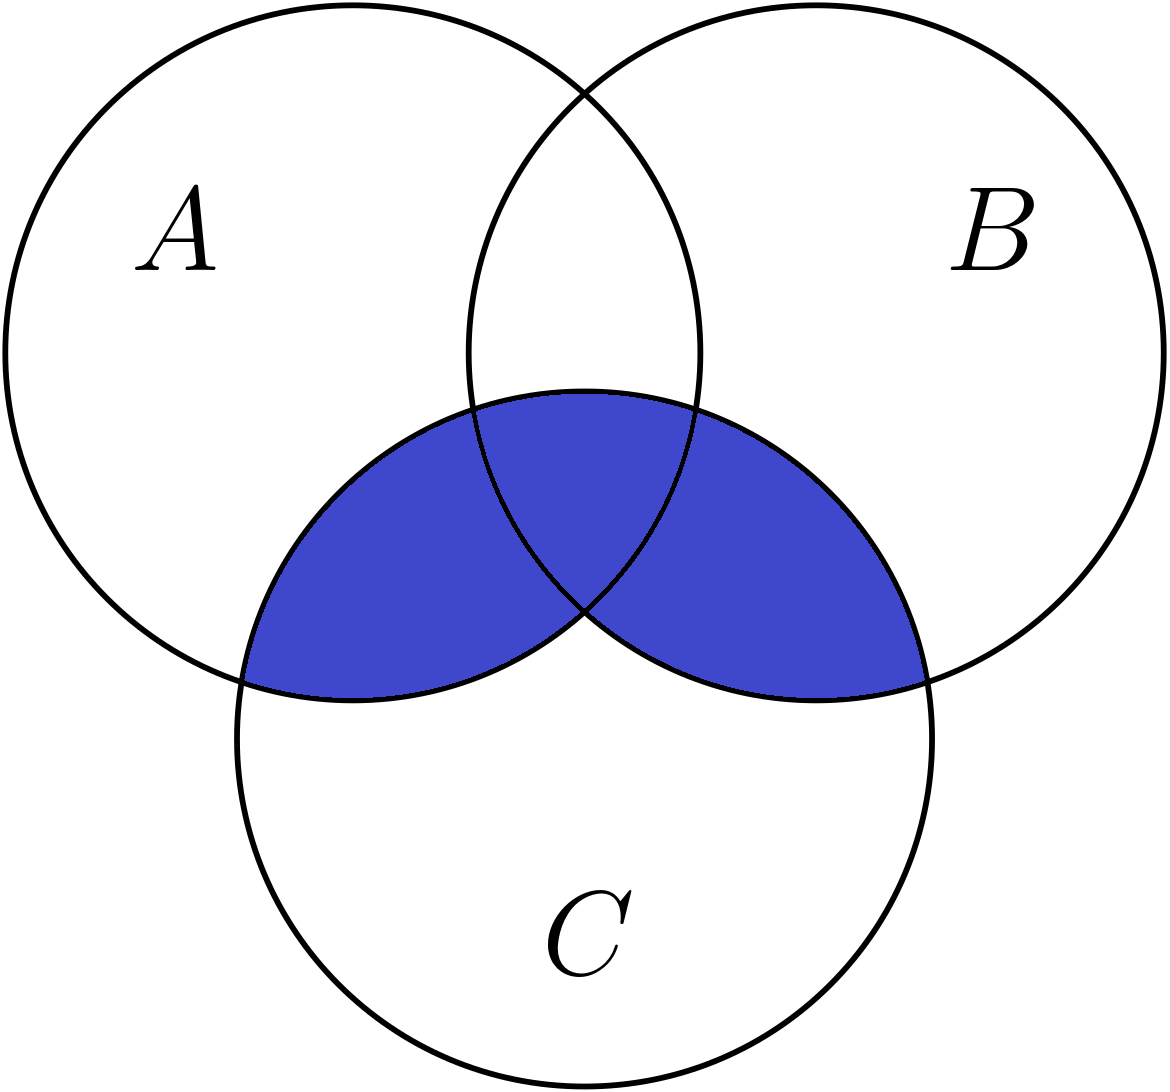
\includegraphics[width = 0.215\textwidth]{3a.png}
\item $A\cup (B \cap C)$ 
\\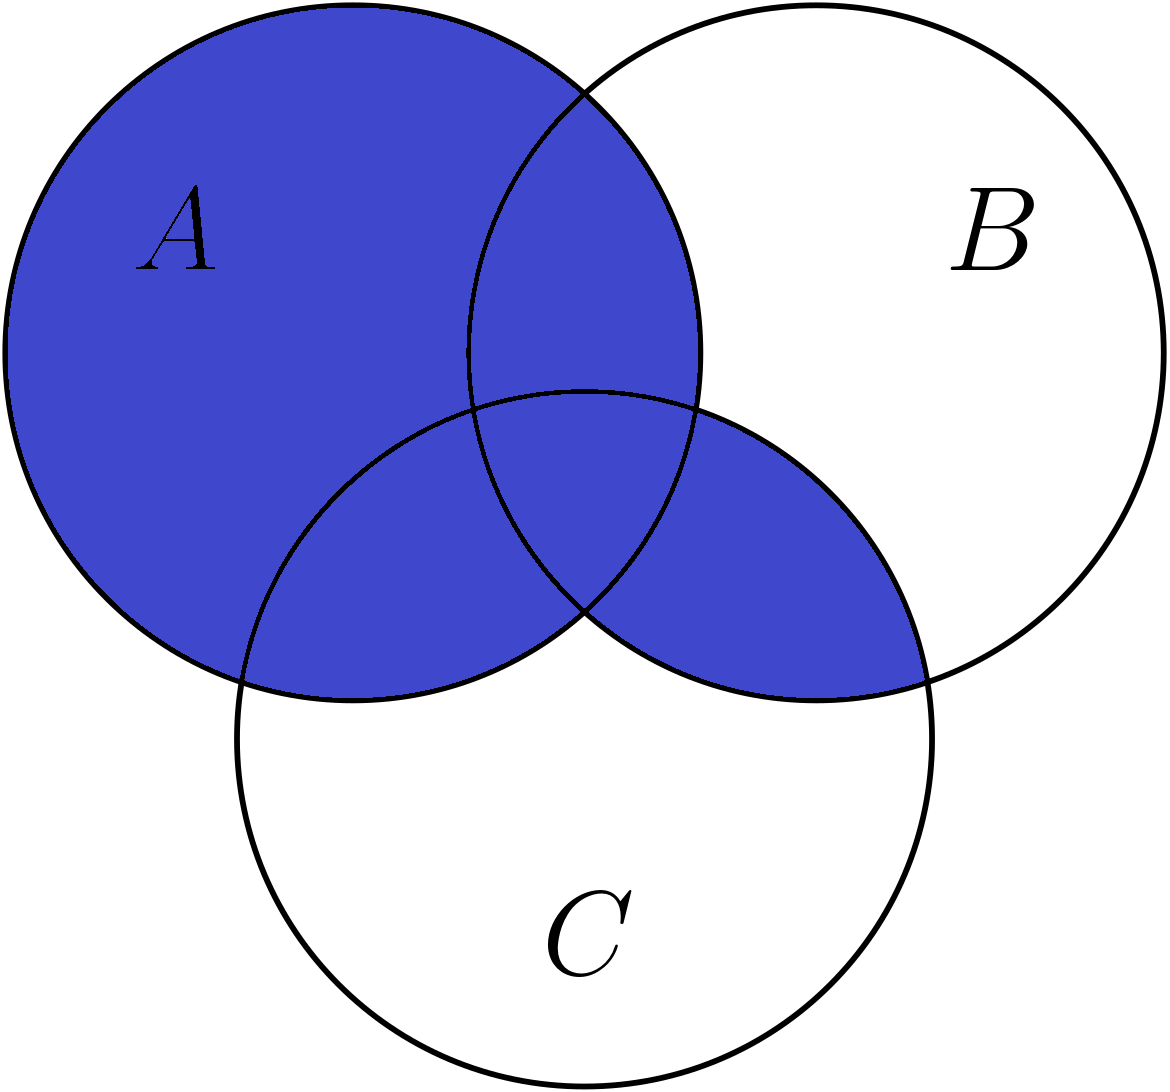
\includegraphics[width = 0.215\textwidth]{3b.png}
\item $\ov{(A \cup B)} \cap C$ 
\\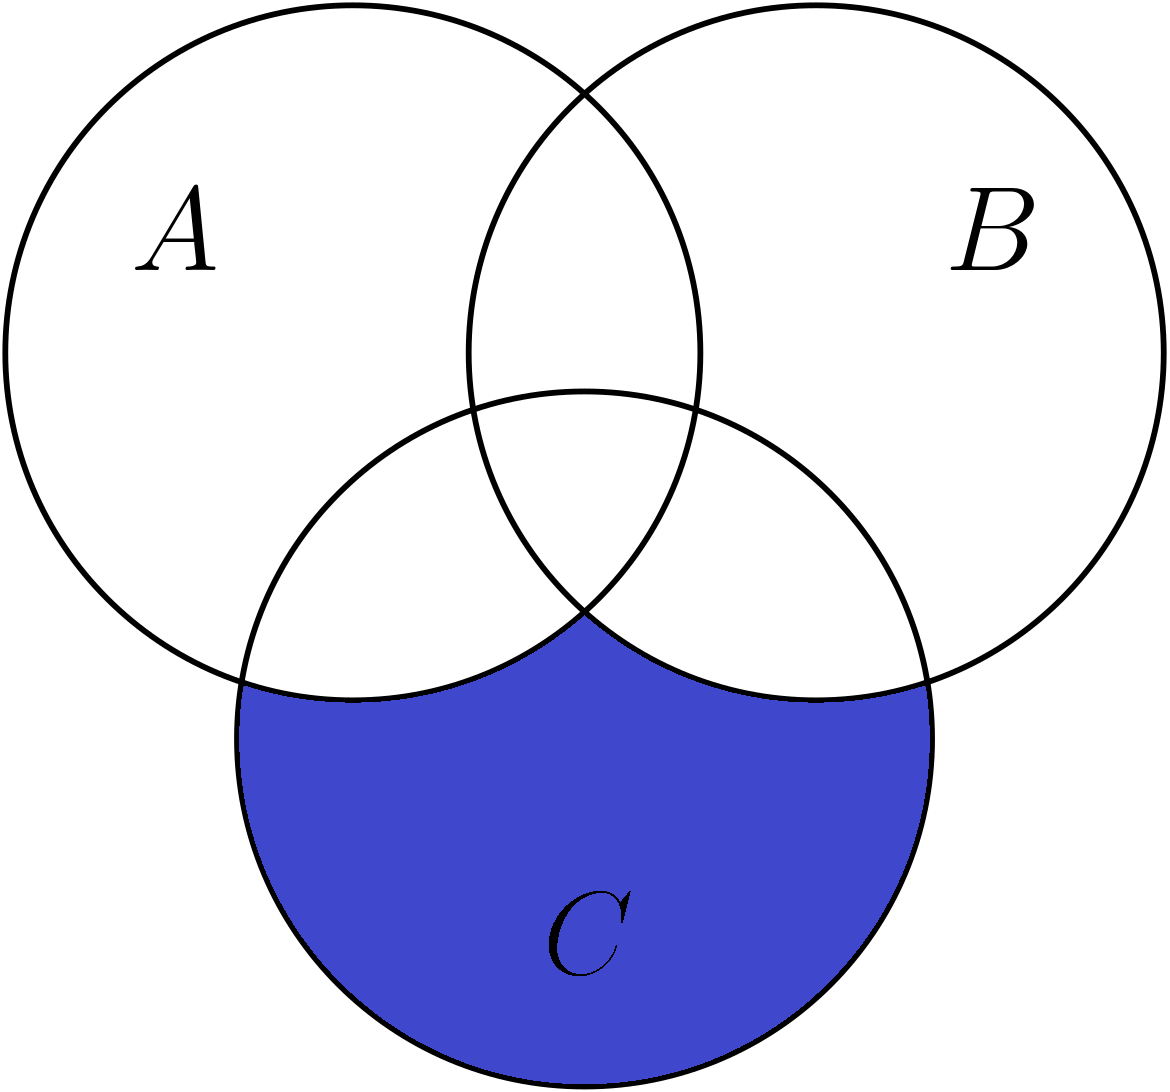
\includegraphics[width = 0.215\textwidth]{3c.png}
\item $\ov{(A - B)} \cap C$
\\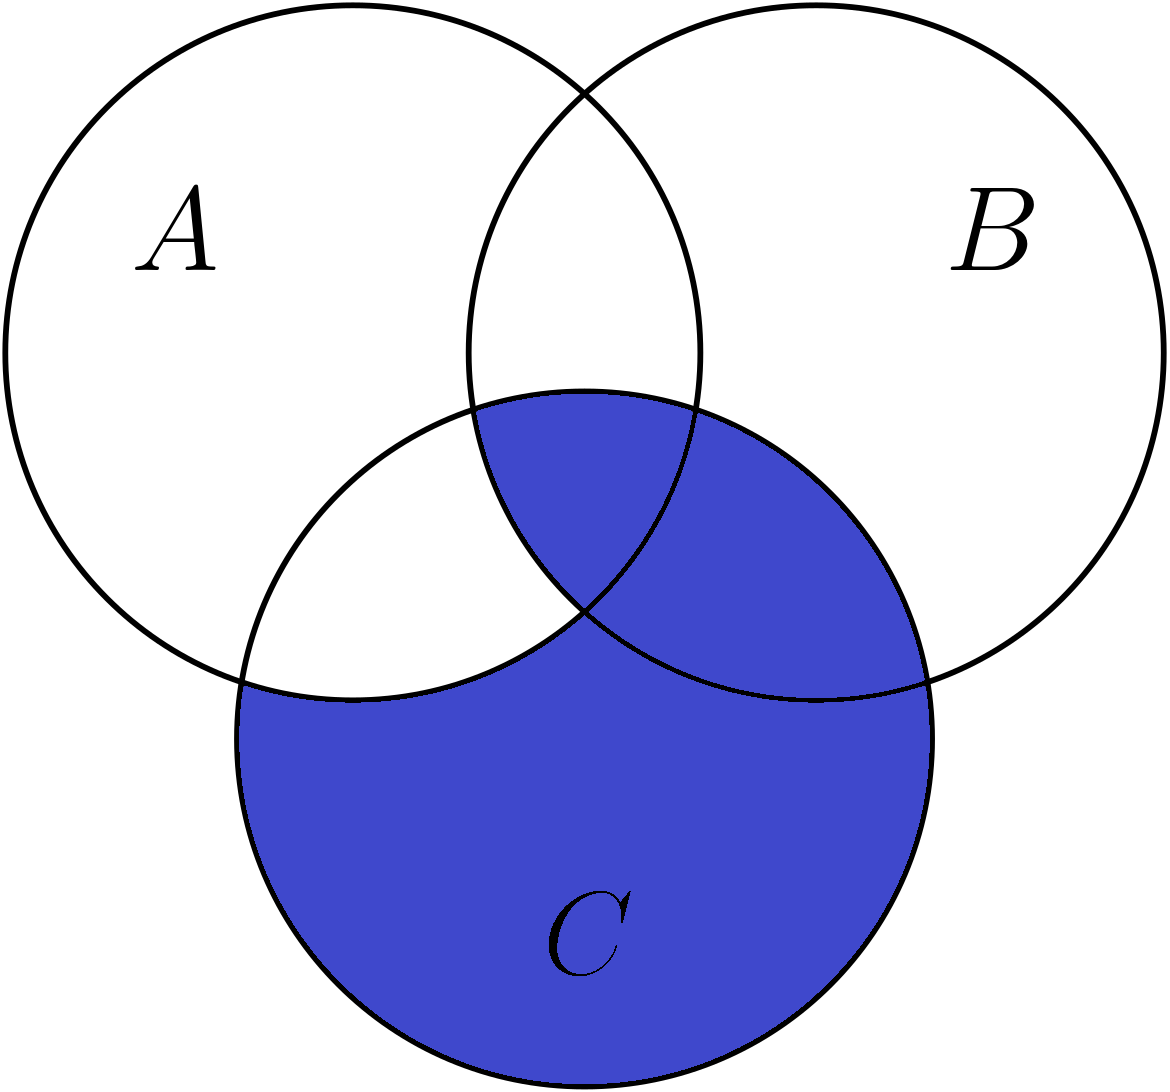
\includegraphics[width = 0.215\textwidth]{3d.png}
\item $(A \cap B) \cup (A \cap \ov{C})$
\\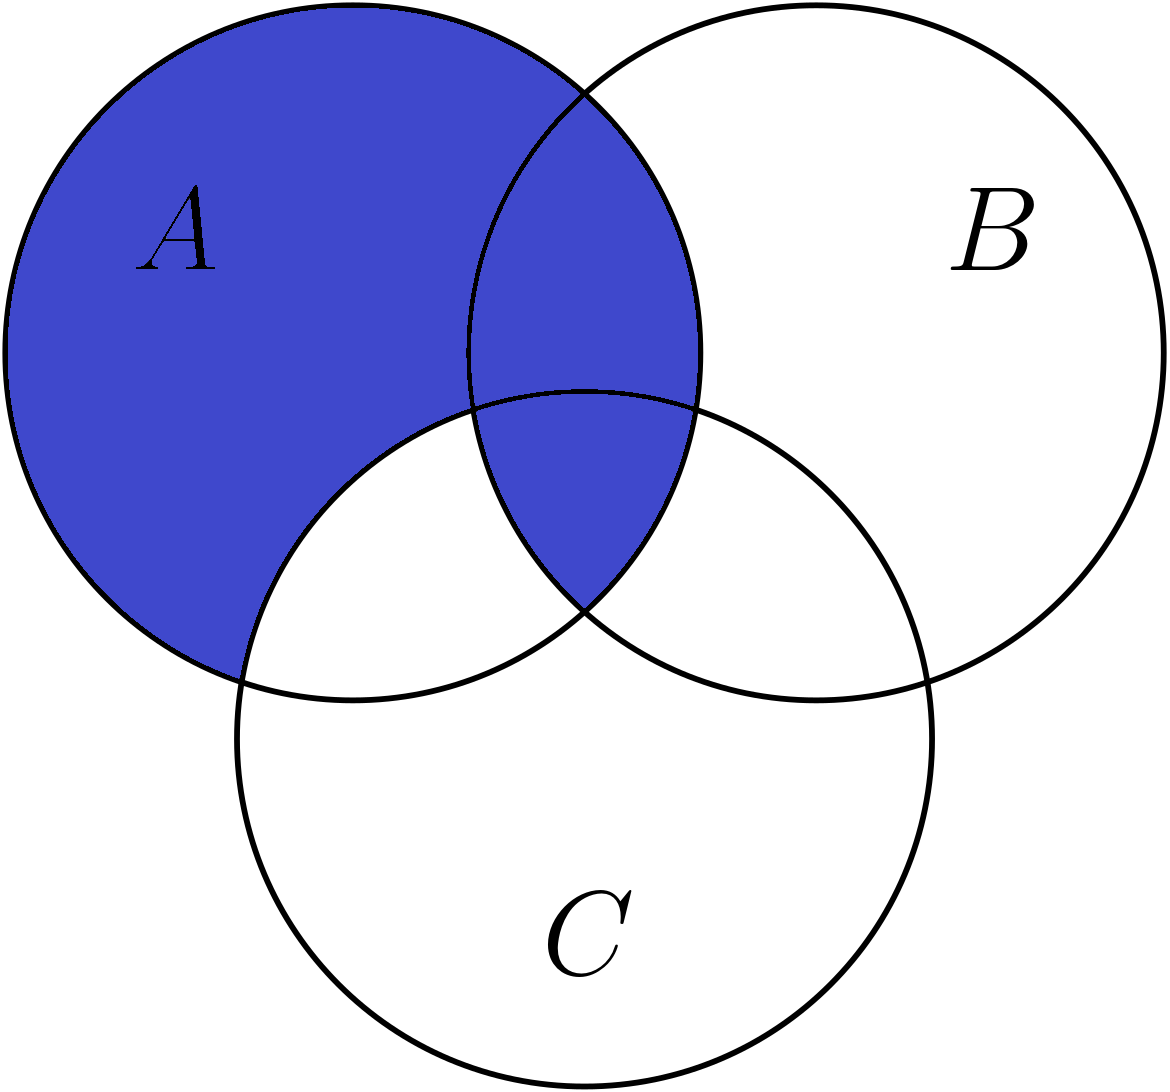
\includegraphics[width = 0.215\textwidth]{3e.png}
\end{enumerate}


\newpage

\item(18pts) Let $A$, $B$ and $C$ be sets. Determine the validity of each statement below. Justify your answer using set identities or membership tables. If two sets are not equivalent, provide a counterexample. A sample solution is provided for part (a).
\begin{enumerate}
\item $A \cap (B-C) = (A-C) \cap B$

\sol{The equation is TRUE. We will show this using set identities. 
\begin{align*}
A \cap (B-C)
 &= A \cap (B \cap \ov{C}) & \text{Difference Equivalence}\\
 &= (A \cap \ov{C}) \cap B & \text{Commutative and Associative Laws}\\
 &= (A - C) \cap B & \text{Difference Equivalence} \\
 \end{align*} 
}

\item $(A-\ov{B}) \cup (B-\ov{A}) = (A \cap B)$ 
\\\sol{The equation is TRUE. We will show this using set identities. 
\begin{align*}
(A-\ov{B}) \cup (B-\ov{A})
 &= (A\cap B) \cup (B\cap A) & \text{Difference Equivalence}\\
 &= (A\cap B) \cup (A\cap B) & \text{Commutative Law}\\
 &= A\cap B & \text{Idempotent Law}\\
 \end{align*} 
}
\item $\ov{(A-B) \cup (B-A)} = \ov{A}\cup B$
\\\sol{The equation is FALSE. We will show this by using a counterexample to find an element that is in one set but not the other.
\\\begin{tabular}{rlll}
\\$\ov{(A-B) \cup (B-A)}$
&$=\ov{(A\cap \ov{B}) \cup (B\cap \ov{A})}$&\text{Difference Equivalence}\\
&$=\ov{(A\cap \ov{B})} \cap \ov{(\ov{A}\cap B)}$&\text{De Morgan's Law, Commutative Law}\\
&$=(\ov{A}\cup B) \cap (A\cup\ov{B})$&\text{De Morgan's Law}\\
\end{tabular}\\\\
let $x$ be an element; $x\in B$\\
then $x\in \ov{A}\cup B$ \quad[def'n of $\cup$]\\
since $x\in \ov{A}$, then $x\not\in A$ \quad[def'n of complement]\\
since $x\in B$, then $x\not\in \ov{B}$ \quad[def'n of complement]\\\\
$\therefore x\not\in (\ov{A}\cup B) \cap (A\cup\ov{B})$, because $x\not\in A\cap\ov{B}$ \quad[def'n of $\cap$]
}\\
\item $((A - B)\cup(A \cap B))\cap((\ov{B\cap \ov{B}}) - A)= \emptyset$
\\\sol{The equation is TRUE. We will show this using set identities. 
\begin{align*}
((A - B)\cup(A \cap B))\cap((\ov{B\cap \ov{B}}) - A)
 &=((A\cap \ov{B})\cup(A \cap B))\cap((\ov{B}\cup B)\cap \ov{A})&\text{De Morgan's Laws}\\
 &=(A\cap (\ov{B}\cup B))\cap((\ov{B}\cup B)\cap \ov{A})&\text{Distributive Laws}\\
 &=(\ov{B}\cup B)\cap (A\cap\ov{A})&\text{Distributive Laws}\\
 &=U\cap\emptyset&\text{Complement Laws}\\
 &=\emptyset&\text{Domination Law}\\
 \end{align*} 
}
\item $A-(B-C) = (A-B)-C$
\\\sol{The equation is FALSE. We will show this by using a counterexample to find an element that is in one set but not the other.
\\Left side:
\begin{align*}
A-(B-C)
 &=A\cap \ov{(B\cap \ov{C})}&\text{Difference Equivalence}\\
 &=A\cap (\ov{B}\cup C)&\text{Morgan's Law}\\
 \end{align*} 
\\Right side:
 \begin{align*}
(A-B)-C
 &=(A\cap\ov{B})\cap\ov{C}&\text{Difference Equivalence}\\
 &=A\cap\ov{B}\cap\ov{C}&\text{Associative Law}\\
 \end{align*} 
let $x$ be an element; $x\in A,B,C$\\
then $x\in A\cap (\ov{B}\cup C)$ \quad[def'n of $\cup$, def'n of $\cap$]\\
since $x\in B$, then $x\not\in \ov{B}$ \quad[def'n of complement]\\
since $x\in C$, then $x\not\in \ov{C}$ \quad[def'n of complement]\\\\
$\therefore x\not\in A\cap\ov{B}\cap\ov{C}$, because $x\not\in \ov{B}\cap\ov{C}$ \quad[def'n of $\cap$]
}\\
\item $(B \cup C)-(A \cup \ov{C}) = \ov{A} \cap C = \ov{A} \cap (A \cup C)$
\\\sol{The equation is TRUE. We will show this using set identities.
\\Let $L.S.=(B \cup C)-(A \cup \ov{C})$
\\Let $R.S.=\ov{A} \cap (A \cup C)$
\\Let $M.S.=\ov{A} \cap C$
\\\\L.S.:
\begin{align*}
(B \cup C)-(A \cup \ov{C})
 &=(B \cup C)\cap\ov{(A \cup \ov{C})}&\text{Difference Equivalence}\\
 &=(B \cup C)\cap (\ov{A} \cap C)&\text{De Morgan's Law}\\
 &=\ov{A} \cap (C\cap (B \cup C))&\text{Associative Law, Commutative Law}\\
 &=\ov{A} \cap C&\text{Absorption Law}\\
 \end{align*} 
\\\\R.S.:
\begin{align*}
\ov{A} \cap (A \cup C)
 &=(\ov{A} \cap A) \cup (\ov{A} \cap C)&\text{Distributive Law}\\
 &=\emptyset \cup (\ov{A} \cap C)&\text{Complement Law}\\
 &=\ov{A} \cap C&\text{Identity Law}\\
 \end{align*} 
\\\\$\therefore L.S.=M.S.=R.S.=\ov{A} \cap C$; The equation is true.
}

\item $(A \cup \ov{C})- (B \cup C) = A \cap B \cap \ov{C}$
\\\sol{The equation is FALSE. We will show this by using a counterexample to find an element that is in one set but not the other.
\\Left side:
\begin{align*}
(A \cup \ov{C})- (B \cup C)
 &=(A \cup \ov{C})\cap \ov{(B \cup C)}&\text{Difference Equivalence}\\
 &=(A \cup \ov{C})\cap (\ov{B} \cap \ov{C})&\text{Morgan's Law}\\
 &=\ov{B} \cap \ov{C}\cap (A \cup \ov{C})&\text{Associative Law, Commutative Law}\\
 &=\ov{B} \cap \ov{C}&\text{Absorption Law}\\
 \end{align*}
let $x$ be an element; $x\in (A-(B\cup C))$\\
then $x\in \ov{B} \cap \ov{C}$ \quad[def'n of $\cap$]\\
since $x\in \ov{B}$, then $x\not\in B$ \quad[def'n of complement]\\
since $x\in \ov{C}$, then $x\not\in C$ \quad[def'n of complement]\\\\
$\therefore x\not\in A \cap B \cap \ov{C}$, because $x\not\in B$ \quad[def'n of $\cap$]
}\\

\end{enumerate}

\newpage

\item(10pts) Determine whether $f$ is a function or not. Justify your answer. Recall, that $\mathbb{R}$ is the set of all real numbers, $\mathbb{Z}$ is the set of all integers. 

\begin{enumerate}
\item $f:\mathbb{R} \rightarrow \mathbb{R}$, $f(x)=\frac{1}{3-x}$.
\\\sol{NO, because $f(3)=\frac{1}{0}\not\in\mathbb{R}$.
}
\item $f:\mathbb{R} \rightarrow \mathbb{R}$, $f(x)=\pm \sqrt{x^2+5}$.
\\\sol{NO, because every element in the domain has up to 2 images.
\\E.g. $f(0)=\begin{cases}\sqrt{5}\\-\sqrt{5}\end{cases}$.
}
\item $f:\mathbb{Z} \rightarrow \mathbb{R}$, $f(x)=\sqrt{x^2+8}$.
\\\sol{YES, because every element in the domain maps to one element in the codomain. $\sqrt{x^2+8}$ is always a real number for any integer input $x$.
}
\item $f:\mathbb{R} \rightarrow \mathbb{R}$, $f(x)=\sqrt{x+1}$.
\\\sol{NO, because there exists elements in the domain that do not map to an element in the codomain.
\\E.g. $f(-2)=\sqrt{-1}\not\in\mathbb{R}$
}
\item $f:\mathbb{R} \rightarrow \mathbb{Z}$, $f(x)=\lceil x \rceil$. Note that $f$ is the ceiling function.
\\\sol{YES, because every element in the domain maps to one element in the codomain. $\lceil x \rceil$ is always an integer for any real number input $x$.
}
\end{enumerate}

\newpage

\item(21pts) For each of the following functions $f:\mathbb{R} \rightarrow \mathbb{R}$ prove or disprove the following:
\begin{itemize}
\item The function is injective (one-to-one).
\item The function is surjective (onto).
\item The function is bijective (both injective and surjective). If the function is a bijection, find its inverse.
\end{itemize}

\begin{enumerate}	
\item $f(x) = \lfloor 3 x \rfloor$. Note that $\lfloor x \rfloor$ is the \textbf{floor} function.
\\\sol{This function is injective, not surjective, not bijective.
\\\\Injective?
\\Assume that $f(x_1)=f(x_2)$. Show that $x_1=x_2$.
\begin{align*}
\lfloor 3 x_1 \rfloor&=\lfloor 3 x_2 \rfloor&\text{}\\
3 x_1&=3 x_2&\text{}\\
x_1&=x_2&\text{}
\end{align*}
$\therefore f(x)$ is injective.
\\\\Surjective?
\\Let $y=1.4$
\\There is no $x\in\mathbb{R}$ such that $f(x)=\lfloor 3 x \rfloor=1.4=y$, because $\lfloor 3 x \rfloor\in\mathbb{Z}$ and $y\not\in\mathbb{Z}$.
\\$\therefore f(x)$ is NOT surjective.
\\\\Bijective?
\\$f(x)$ is not surjective.
\\$\therefore f(x)$ is NOT bijective.
}\\
\item $f(x) = 8-3x$
\\\sol{This function is injective, surjective, bijective.
\\\\Injective?
\\Assume that $f(x_1)=f(x_2)$. Show that $x_1=x_2$.
\begin{align*}
8-3x_1&=8-3x_2&\text{}\\
-3x_1&=-3x_2&\text{}\\
x_1&=x_2&\text{}
\end{align*}
$\therefore f(x)$ is injective.
\\\\Surjective?
\\Let $y$ be an arbitrary image.
\begin{align*}
y&=8-3x&\text{}\\
y-8&=-3x&\text{}\\
\frac{y-8}{-3}&=x&\text{}
\end{align*}
For any $y\in\mathbb{R}$: $\frac{y-8}{-3}\in\mathbb{R}$
\\We found an element $x=\frac{y-8}{-3}\in\mathbb{R}$ such that $f(x)=f(\frac{y-8}{-3})=8-3(\frac{y-8}{-3})=y$
\\$\therefore f(x)$ is surjective.
\\\\Bijective?
\\$f(x)$ is injective and surjective.
\\$\therefore f(x)$ is bijective.
\\Inverse:
\\$f^{-1}(y)=\frac{y-8}{-3}$
}\\
\item $f(x) = |8 - 3 x|$
\\\sol{This function is not injective, not surjective, not bijective.
\\\\Injective?
\\Assume that $f(x_1)=f(x_2)$. Show that $x_1=x_2$.
\begin{align*}
|8-3x_1|&=|8-3x_2|&\text{}\\
8-3x_1&=\pm(8-3x_2)&\text{}\\
-3x_1&=\pm(8-3x_2)-8&\text{}\\
x_1&=\frac{\pm(8-3x_2)-8}{-3}&\text{}\\
x_1&=\begin{cases}\frac{(8-3x_2)-8}{-3}=x_2&\text{}\\\frac{-(8-3x_2)-8}{-3}=\frac{16}{3}-x_2&\text{$x_1\neq x_2$}\end{cases}
\end{align*}
$\therefore f(x)$ is NOT injective.
\\\\Surjective?
\\Let $y=-1$
\\There is no $x\in\mathbb{R}$ such that $f(x)=|8 - 3 x|=-1=y$, because $|8 - 3 x|$ does not have images in codomain $\mathbb{R}<0$.
\\$\therefore f(x)$ is NOT surjective.
\\\\Bijective?
\\$f(x)$ is not injective or surjective.
\\$\therefore f(x)$ is NOT bijective.
}\\
\item $f(x) = 4x^3 + 5$
\\\sol{This function is injective, surjective, bijective.
\\\\Injective?
\\Assume that $f(x_1)=f(x_2)$. Show that $x_1=x_2$.
\begin{align*}
4{x_1}^3 + 5&=4{x_2}^3 + 5&\text{}\\
4{x_1}^3&=4{x_2}^3&\text{}\\
{x_1}^3&={x_2}^3&\text{}\\
x_1&=x_2&\text{}
\end{align*}
$\therefore f(x)$ is injective.
\\\\Surjective?
\\Let $y$ be an arbitrary image.
\begin{align*}
y&=4x^3 + 5&\text{}\\
y-5&=4x^3&\text{}\\
\frac{y-5}{4}&=x^3&\text{}\\
\sqrt[3]{\frac{y-5}{4}}&=x&\text{}
\end{align*}
For any $y\in\mathbb{R}$: $\sqrt[3]{\frac{y-5}{4}}\in\mathbb{R}$
\\We found an element $x=\sqrt[3]{\frac{y-5}{4}}\in\mathbb{R}$ such that $f(x)=f(\sqrt[3]{\frac{y-5}{4}})=4(\sqrt[3]{\frac{y-5}{4}})^3 + 5=y$
\\$\therefore f(x)$ is surjective.
\\\\Bijective?
\\$f(x)$ is injective and surjective.
\\$\therefore f(x)$ is bijective.
\\Inverse:
\\$f^{-1}(y)=\sqrt[3]{\frac{y-5}{4}}=x$
}\\
\item $f(x) = 2x^2-3$
\\\sol{This function is not injective, not surjective, not bijective.
\\\\Injective?
\\Assume that $f(x_1)=f(x_2)$. Show that $x_1=x_2$.
\begin{align*}
2{x_1}^2-3&=2{x_2}^2-3&\text{}\\
2{x_1}^2&=2{x_2}^2&\text{}\\
{x_1}^2&={x_2}^2&\text{}\\
{x_1}&=\pm\sqrt{{x_2}^2}&\text{}\\
{x_1}&=\pm x_2&\text{}\\
x_1&=\begin{cases}x_2&\text{}\\-x_2&\text{$x_1\neq x_2$}\end{cases}
\end{align*}
$\therefore f(x)$ is NOT injective.
\\\\Surjective?
\\Let $y=-4$
\\There is no $x\in\mathbb{R}$ such that $f(x)=2x^2-3=-4=y$, because $2x^2-3$ does not have images in codomain $\mathbb{R}<-3$.
\\$\therefore f(x)$ is NOT surjective.
\\\\Bijective?
\\$f(x)$ is not injective or surjective.
\\$\therefore f(x)$ is NOT bijective.
}\\
\end{enumerate}

\newpage

\item(9pts) Let $f$ and $g$ both be functions from real numbers to real numbers. Let $f(x) = 3x^2-8$ and $g(x) = x-2$. Define each of the following, simplify, and then evaluate. You need to show your work.
\begin{enumerate}
\item $(f\circ g) (x= -1)$ 
\\\sol{
\begin{align*}
(f\circ g)(x=-1)&=f(g(x))&\text{}\\
&=3(x-2)^2-8&\text{}\\
&=3((-1)-2)^2-8&\text{}\\
&=3(-3)^2-8&\text{}\\
&=3(9)-8&\text{}\\
&=27-8&\text{}\\
&=19&\text{}\\
\end{align*}
}
\item $(g\circ f)(x=2)$
\\\sol{
\begin{align*}
(g\circ f)(x=2)&=g(f(x))&\text{}\\
&=(3x^2-8)-2&\text{}\\
&=(3(2)^2-8)-2&\text{}\\
&=(3(4)-8)-2&\text{}\\
&=(4)-2&\text{}\\
&=2&\text{}\\
\end{align*}
}
\item $((g\circ f)\circ g) (x=1)$ Reuse solution to part (b).
\\\sol{
\begin{align*}
(g\circ f)&=(3x^2-8)-2&\text{from (b)}\\
((g\circ f)\circ g) (x=1)&=(3(g(x))^2-8)-2&\text{}\\
&=(3(x-2)^2-8)-2&\text{}\\
&=3(x-2)^2-10&\text{}\\
&=3((1)-2)^2-10&\text{}\\
&=3(-1)^2-10&\text{}\\
&=3(1)-10&\text{}\\
&=-7&\text{}\\
\end{align*}
}
\end{enumerate}

\newpage

\item (8 pts) Let $f:\mathbb{R} \rightarrow \mathbb{R}$ and $g:\mathbb{R} \rightarrow \mathbb{R}$. Prove or disprove the followings:

\begin{enumerate}
\item if $f$ and $g$ are both bijections, then $f(x)+g(x)$ is also a bijection. 
\\\sol{FALSE. We will disprove using a counterexample:
\\let f(x)=x; f is a bijection
\\let g(x)=-x; g is a bijection
\begin{align*}
f(x)+g(x)
&=x+(-x)\\
&=0&\text{}\\
\end{align*}
\\Let $y=1$
\\There is no $x\in\mathbb{R}$ such that $f(x)+g(x)=x+(-x)=1=y$, because $x+(-x)=0$; it does not have images in codomain $\mathbb{R}\neq0$.
\\$\therefore f(x)+g(x)$ is NOT surjective.
\\$\therefore f(x)+g(x)$ is NOT bijective.
}
\item if $f$ is a bijection, then for any real number $c \neq 0$, $c \cdot f(x)$ is also a bijection.
\\\sol{TRUE. $c\cdot f(x)$ is bijective.
\\\\Injective?
\\Assume that $c\cdot f(x_1)=c\cdot f(x_2)$, $c\neq 0$. Show that $x_1=x_2$.
\begin{align*}
c\cdot f(x_1)&=c\cdot f(x_2)&\text{}\\
f(x_1)&=f(x_2)&\text{}\\
x_1&=x_2&\text{$f(x)$ has 1 and only 1 preimage for all $f(x)\in\mathbb{R}$}
\end{align*}
$\therefore c\cdot f(x)$ is injective.
\\\\Surjective?
\\Let $y$ be an arbitrary image.
\begin{align*}
y&=c\cdot f(x)&\text{}\\
\frac{y}{c}&=f(x)&\text{}\\
f^{-1}(\frac{y}{c})&=x&\text{}\\
\end{align*}
For any $y\in\mathbb{R}$: $f^{-1}(\frac{y}{c})\in\mathbb{R}, c\neq 0$
\\We found an element $x=f^{-1}(\frac{y}{c})\in\mathbb{R}$ such that $c\cdot f(x)=c\cdot f(f^{-1}(\frac{y}{c}))=c\cdot f(f^{-1}(\frac{y}{c}))=y$
\\$\therefore c\cdot f(x)$ is surjective.
\\\\Bijective?
\\$c\cdot f(x)$ is injective and surjective.
\\$\therefore c\cdot f(x)$ is bijective.
}
\end{enumerate}
 
\end{enumerate}
\end{document}